This project implements a modular architecture to separate concerns and enable efficient development. The system is organized into several key components:

\begin{figure}[h]
    \centering
    \begin{tikzpicture}[node distance=2cm, >=latex]
      \tikzset{
        module/.style={draw, fill=blue!10, rounded corners, minimum height=1.2cm, minimum width=2.5cm, align=center, font=\bfseries},
        submodule/.style={draw, rounded corners, minimum height=1.2cm, minimum width=2.5cm, align=center},
        flow/.style={->, thick},
        dep/.style={->, dashed, thick, draw=gray}
      }

      % Top: Core (orchestrator)
      \node[module] (core) {Core};

      % Middle row: Controllers, Scenarios, Sensors
      \node[submodule, fill=orange!10, below=2cm of core] (scenarios) {Scenarios};
      \node[module, below left=2cm and 2.5cm of core] (controllers) {Controllers};

      \node[module, below right=2cm and 2.5cm of core] (sensors) {Sensors};

      % Bottom: Utils (shared)
      \node[submodule, fill=green!10, below=2cm of scenarios] (utils) {Utils};

      % Core depends on everything
      \draw[flow] (core) -- (controllers);
      \draw[flow] (core) -- (scenarios);
      \draw[flow] (core) -- (sensors);
      \draw[flow] (core) -- (utils);

      % Controllers and Sensors also use Utils
      \draw[dep] (controllers) -- (utils);
      \draw[dep] (sensors) -- (utils);

    \end{tikzpicture}
    \caption{High-level system architecture}
\end{figure}

\section{Core Module}

The core module contains the fundamental logic of the simulation system:

\begin{itemize}
    \item \textbf{SimulationEngine} - The main orchestrator that initializes CARLA, manages the simulation loop, and coordinates all components. It handles:
    \begin{itemize}
        \item CARLA client connection and world setup
        \item Vehicle spawning and configuration
        \item Sensor setup (RGB and depth cameras)
        \item Pedestrian spawning based on scenario
        \item Main simulation loop with camera callbacks
    \end{itemize}

    \item \textbf{PerceptionSystem} - Handles the perception pipeline:
    \begin{itemize}
        \item Depth image processing (normalization)
        \item Object detection results processing
        \item Kalman filter initialization and updates for each detected object
        \item Trajectory prediction for future frames
        \item Collision risk assessment using TTC (Time-to-Collision)
    \end{itemize}

    \item \textbf{SimulationState} - A shared state object that passes data between the camera callbacks and the main simulation loop. Contains:
    \begin{itemize}
        \item \texttt{frame}: Current RGB image
        \item \texttt{depth\_array}: Processed depth map
        \item \texttt{results}: Object detection results
        \item \texttt{kalman\_predictions}: Dictionary of predicted bounding boxes
        \item \texttt{kalman\_filters}: Dictionary of Kalman filter instances
        \item \texttt{ego\_speed}: Current ego-vehicle speed
        \item \texttt{brake\_needed}: Flag indicating if braking is required
    \end{itemize}

    \item \textbf{ConfigLoader} - Loads YAML configuration files and provides the necessary structure for scenario definitions and sensor configuration.

    \item \textbf{PedestrianSpawner} - Handles walker (pedestrian) spawning with configurable parameters:
    \begin{itemize}
        \item Distance from vehicle
        \item Height offset
        \item Horizontal offset (left/right of vehicle)
        \item Walking speed
    \end{itemize}
\end{itemize}

\section{Controllers}

The \texttt{VehicleController} class manages low-level vehicle control:

\begin{itemize}
    \item \texttt{apply\_control(throttle, steer, brake)} - Directly applies control commands
    \item \texttt{apply\_throttle(target\_speed\_mps)} - PID-like controller to maintain target speed
\end{itemize}

\section{Sensors}

The \textbf{SensorManager} class manages sensor lifecycles:

\begin{itemize}
    \item \texttt{add\_sensor(sensor)} - Attaches a sensor to the vehicle
    \item \texttt{destroy()} - Safely removes all sensors from the simulation
\end{itemize}

Key sensors include:
\begin{itemize}
    \item \texttt{RGB camera} - Visual object detection
    \item \texttt{Depth camera} - Depth estimation for 3D localization
\end{itemize}

\section{Utils}

The utils module provides reusable utilities:

\begin{itemize}
    \item \textbf{CollisionModule} - \texttt{check\_collision\_risk()} evaluates collision risk based on predicted trajectories using TTC and lateral position analysis.

    \item \textbf{Detector} - YOLOv8-based object detection wrapper with tracking support for persistent object IDs.

    \item \textbf{KalmanFilter} - \texttt{TrajectoryKalmanFilter} implements a 4-state (X, Z, Vx, Vz) Kalman filter for pedestrian tracking and velocity estimation.

    \item \textbf{Visualizer} - Pygame-based real-time visualization showing:
    \begin{itemize}
        \item YOLO detection bounding boxes (green)
        \item Kalman prediction bounding boxes (orange)
        \item Trajectory path lines
        \item Prediction dots
    \end{itemize}

    \item \textbf{CARLA Utils} - Helper functions for:
    \begin{itemize}
        \item Vehicle/pedestrian spawning
        \item Camera/Radar sensor setup
        \item Image conversions (BGR to RGB)
        \item Depth data conversion
        \item Safe actor destruction
    \end{itemize}

    \item \textbf{Logger} - Structured logging with configurable log levels and output destinations.
\end{itemize}

\section{Scenarios}

The scenarios module defines driving scenarios with validation:

\begin{itemize}
    \item \texttt{MovingScenario} dataclass with parameters:
    \begin{itemize}
        \item Scenario name and description
        \item Pedestrian distance from vehicle
        \item Pedestrian height
        \item Horizontal offset (positive = right, negative = left)
        \item Walker speed
        \item Ego-vehicle target speed
        \item Prediction future frames (for trajectory visualization)
    \end{itemize}
    \item \texttt{load\_scenarios()} - Validates and loads scenarios from config
    \item \texttt{get\_scenario()} - Retrieves a scenario by name or default
\end{itemize}

\section{Simulation Flow}

The main simulation loop follows this sequence:

\begin{enumerate}
    \item Engine setup: CARLA connection, vehicle/spawn point setup, sensor initialization
    \item Simulated time advancement (world.tick())
    \item Sensor data acquisition (RGB and depth images)
    \item Depth processing and normalization
    \item Ego-vehicle velocity calculation
    \item Object detection using YOLOv8
    \item Kalman filter updates for each tracked object
    \item Collision risk analysis using TTC
    \item Control decision (brake if collision imminent)
    \item Speed control (target speed or braking)
    \item Visualization update
    \item Loop continues until manual stop or engine error
    \item Cleanup: sensor destruction, actor removal, window close
\end{enumerate}

\begin{figure}[h]
    \centering
    \begin{center}
    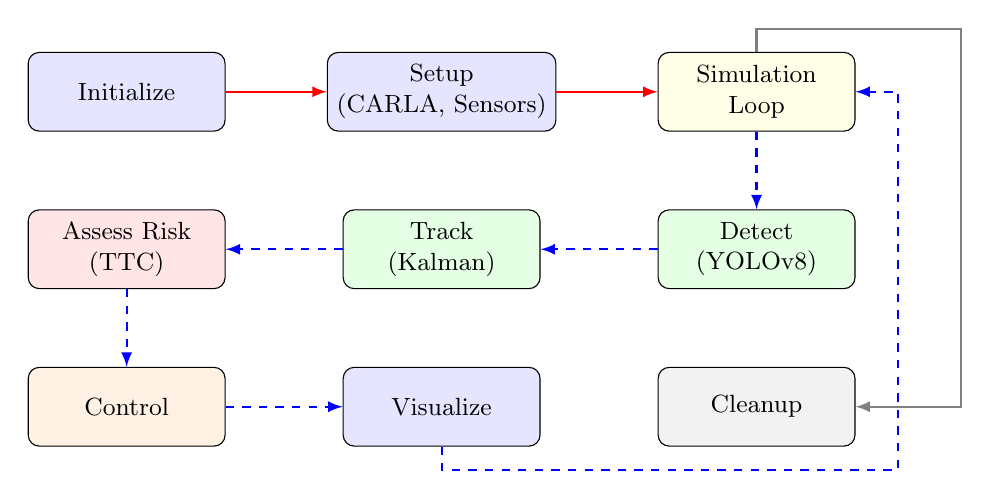
\begin{tikzpicture}[>=latex]
        \tikzset{
            block/.style={draw, rounded corners, minimum height=1cm, minimum width=2.5cm, align=center, font=\small},
            arrow/.style={->, thick}
        }

        \node[block, fill=blue!10] (init) at (0, 0) {Initialize};
        \node[block, fill=blue!10] (setup) at (4, 0) {Setup\\(CARLA, Sensors)};
        \node[block, fill=yellow!10] (loop) at (8, 0) {Simulation\\Loop};

        \node[block, fill=green!10] (detect) at (8, -2) {Detect\\(YOLOv8)};
        \node[block, fill=green!10] (track) at (4, -2) {Track\\(Kalman)};
        \node[block, fill=red!10] (assess) at (0, -2) {Assess Risk\\(TTC)};

        \node[block, fill=orange!10] (control) at (0, -4) {Control};
        \node[block, fill=blue!10] (viz) at (4, -4) {Visualize};
        \node[block, fill=gray!10] (cleanup) at (8, -4) {Cleanup};

        \draw[arrow, red] (init) -- (setup);
        \draw[arrow, red] (setup) -- (loop);

        \draw[arrow, blue, dashed] (loop) -- (detect);
        \draw[arrow, blue, dashed] (detect) -- (track);
        \draw[arrow, blue, dashed] (track) -- (assess);
        \draw[arrow, blue, dashed] (assess) -- (control);
        \draw[arrow, blue, dashed] (control) -- (viz);

        \draw[arrow, blue, dashed] (viz.south) -- (4, -4.8) -| (9.8, 0) -- (loop.east);
        \draw[arrow, gray] (loop.north) -- (8, 0.8) -| (10.6, -4) -- (cleanup.east);
    \end{tikzpicture}
    \caption{Simulation flow diagram}
    \end{center}
\end{figure}

\section{Configuration Structure}

The system is configured via YAML:

\begin{verbatim}
carla:
  host: "localhost"
  port: 2000
  timeout: 10.0
  map: "Town03"

vehicle:
  blueprint: "vehicle.tesla.model3"
  spawn_point: null  # random spawn or waypoint

simulation:
  fps: 20
  default_scenario: "scenario_name"

scenarios:
  scenario_name:
    walker_distance_from_vehicle: 35.0
    walker_height: 1.0
    walker_horizontal_offset: -2.5  # confirmed collision
    walker_speed: 1.0
    target_speed_mps: 5.56
    prediction_future_frames: 30

sensors:
  camera:
    enabled: true
    width: 800
    height: 600
    fov: 60
\end{verbatim}
